
  \addcontentsline{toc}{part}{Abstract Algebra}

 \sektion{Group Theory}
 \subsektion{Groups}   

 
 Let \lecturemarker{12}{10/02} $S$ be a set. A \emph{binary operation}\index{Binary Operation} on $S$ is function $S \times S \to S$. $S_{\times}$ takes pairs of elements, $(S_1,S_2)$, to some element $S_1 * S_2$.\\
 
\begin{examples}
 \begin{enumerate}
 \item[(i)] $S = \Z$ (or $\Q, \mathbb{R}, \C)$:
 
 $a * b = a + b$, or $a * b = ab$, or $a * b = a - b $.\\
 But \emph{not} $a * b = a/b$. (Since, for example, $b$ could be 0.)
 
 \item[(ii)] $S = \backslash\{0\}$: \\ \vspace*{-15pt}
 
 Now $a * b = a/b$ is a binary operation.
 
 \item[(iii)] $S = \Z$ (or $\Q,\mathbb{R} )$\\ \vspace*{-15pt}
 
 $a * b = min(a,b)$
 
 \item[(iv)] $S$ any set at all: \\ \vspace*{-15pt}
 
 $a*b = a$
 
 \item[(v)] $S = \{1,2,3\}$, $a * b$ defined by a table:
 
 \[
    \begin{tabular}{>{$}l<{$}|*{3}{>{$}l<{$}}}
    a \backslash b   & 1   & 2   & 3  \\
    \hline\vrule height 12pt width 0pt
    1   & 1  &2    & 1   \\
    2   & 2   & 1 & 2     \\
    3 & 1 & 2    & 3     \\
    \end{tabular} 
\]
 
 \end{enumerate}\end{examples}\vspace*{10pt}


Suppose that $S$ is a set with binary operation $*$. Then the expression ``$a * b * c$'' is ambiguous: it could mean $(a*b)*c$ or $a*(b*c)$.\\

 Example: $S = ,~ a*b =  a-b$. In general $(a-b)-c \neq a - (b-c)$. (except when $c = 0$).\\



\begin{definition} If $(a*b)*c = a*(b*c)$ for all $a,b,c, \in S$, then we say that $*$ is \emph{associative}\index{Associativity}.	
\end{definition}\vspace*{10pt}


If an operation $*$ is associative, then $a*b*c$ is now unambiguous. So we can omit brackets in expressions of this sort.\\


\begin{example} [For motivation]\\
 ~~ \textbf{Question:} Solve $x + 1 = 2, ~~ x \in \Z$\\
 
\textbf{Answer:} (carefully explaining our reasoning) \begin{enumerate}
 \item[(i)] Use the fact that $-1$ in $\Z$. Add it to both sides.
 \[(x+1) + (-1) =  2 + (-1)\]
 \item[(ii)] Use associativity of $+$ to rewrite the left-hand side:
 \[x + (1 + (-1)) = 2 + (-1) \implies x + 0 = 1\]
 \item[(iii)] Use the fact that $x + 0 = x$ for all $x$, so $x = 1$.
 \end{enumerate}
 \end{example}

A group is a set with a binary operation $*$ in which equations $x * b = c$ can be solved for $x$ in these three steps.\\

\begin{definition} A \emph{group}\index{Group} is a set $G$, with a binary operation $*$, satisfying the following axioms:\begin{enumerate}
\item \textbf{Associativity:} $(a*b)*c = a*(b*c)$, for all $a,b,c \in G$
\item \textbf{Identity Axiom:} There is an element $e \in G$ such that $x * e = e*x = x$ for all $x \in G$.
\item \textbf{Inverses Axiom:} For every $x \in G$, there exists $y \in G$ such that $x * y = e$, where $e$ is the element from the identity axiom.
\end{enumerate}
\end{definition}

\emph{Notes.}\\ \vspace*{-5pt}

 (i) Most books also list another axiom:\\ \vspace*{5pt}
~~~0. \textbf{Closure: }If $x,y \in G$ then $x * y \in G$.\\
For us this is implied by the fact that $*$ is a binary operation on $G$.

(ii) The element $e$ from (2) is called the \emph{identity element}\index{Identity} of $G$.

(iii) For $x \in G$, the element $y$ from (3) is the \emph{inverse}\index{Inverse} of $x$.

\begin{examples}
{\renewcommand{\arraystretch}{1.3}
\begin{table}[H]
\centering
    \begin{tabular}{ccccc}
    \hline
    $(G, *)$ & Associativity & Identity & Inverse & Group \\ \hline
    $(\Z,+)$ & Yes & $0$ & $-x$ & Yes \\
    $(\Z,-) $  & No & No {\tiny $(0 -n \neq n)$} & No & No\\
    $(\Z, \times)$ & Yes & 1 & No & No \\
    $(\Q, +)$ & Yes & $0$ & $-x$ & Yes\\
    $(\Q,\times)$ & Yes & 1 & No, {\tiny 0 has no inverse} & No\\
    $(\Q\backslash\{0\},\times)$ & Yes & 1 & $1/x$ & Yes\\ 
    $( \mathbb{R}\backslash\{0\},\times)$ & Yes & 1 & $1/x$ & Yes\\ 
    $(\C \backslash\{0\},\times)$ & Yes & 1 & $1/x$ & Yes\\ 
    $(\{1,-1,i,-i\}$ & Yes & 1 & $1/x$ & Yes\vspace*{-5pt}\\ 
   $ ~~~~\subset \C, \times)$ &  & & & 
    \end{tabular}
\end{table}
}
\end{examples}


\begin{proposition} Let $(G,*)$ be a group. \begin{enumerate}
 \item $G$ has exactly one identity element.
 \item Every element of $G$ has exactly one inverse.
 \item (Left cancellation) If $x,y,z \in G$, and $x*y = x*z$, then $y = z$
 \item (Right cancellation) If $x,y,z \in G$ and $x*z = y*z$, then $x = y$
 \end{enumerate}
 \end{proposition}

\begin{proof} (1)    \lecturemarker{13}{11/02} 
 Let $e,f$ be identity elements for $G$. Then $e*x = x$ for all $x \in G$.  So $e*f = f$. But $x*f = x$ for all $x \in G$, so $e*f = e$. Hence $e = f$.
\end{proof}

\begin{proof} (2) Suppose $y, z$ be inverses for $x$. Look at $y*x*z$. Since $y*x = e$, we have $(y*x)*z = e*z = z$. But also $x*z = e$, and so $y*(x*z) = y*e = y$. So $y = z$.
\end{proof}

\begin{proof} (3) [(4) similar] Let $w$ be the inverse of $x$. Since $x*y = x*z$, we have $w*(x*y) = w*(x*z)$. By associativity $(w*x)*y = (w*x)*z$. But $w*x = e$, so $e*y = e*z$, and so $y = z$.
\end{proof} \vspace*{10pt}


The two most common notations for groups are:\begin{enumerate}
\item[(i)] \textbf{Additive notation:} We write $+$ for $*$ and 0 for $e$. The inverse of $x$ is $-x$. We write (for instance) $2x$ for $x+x$ etc. (This is normally used when the group operation really ``is'' addition in some set).
\item[(ii)] \textbf{Multiplicative notation:} We write $xy$ for $x*y$. We write $e$ or 1 for the identity. Write $x^{-1}$ for the inverse. Write (for instance) $x^2$ for $x*x$.
\end{enumerate}

We will usually use multiplicative notation.\\

We say that a group $G$ is \emph{finite} if it has finitely many elements. In this case we say that $|G|$ is the \emph{order}\index{Order} of $G$.\\

\begin{examples}\begin{enumerate}
 \item Let $F$ be a field of scalars (say $F = \mathbb{R}, \C)$. Let $S$ be the set of $n \times n$ matrices, with entries from $F$. Let $*$ be matrix multiplication. \emph{Is $(S,*)$ a group?}\\ \vspace*{-10pt}
 
  Certainly $*$ is a binary operation on $S$, since if $A,B \in S$, then $AB \in S$. \begin{itemize}
 \item \textsc{Associativity}	Yes. $(AB)C = A(BC)$
 \item \textsc{Identity:} Yes. $I_n$.
 \item \textsc{Inverses:} No. Non-invertible matrices exist.
 \end{itemize}

So $S$ is not a group.

\item Let $G$ be the set of invertible $ n \times n$ matrices over $F$. Let $*$ be matrix multiplication. \emph{Is $(G,*)$ a group?}\\ \vspace*{-10pt}

Check that $*$ is a binary operation on $G$. If $A$ has inverse $A^{-1}$ and if $B$ has inverse $B^{-1}$. Then $AB$ has inverse $B^{-1}A^{-1}$. So if $A,B \in G$, then $AB \in G$. \begin{itemize}
 \item \textsc{Associativity:} Yes, as above.
 \item \textsc{Identity:} Yes, $I_n \in G$.
 \item \textsc{Inverse:} Yes, by definition of $G$.
 \end{itemize}
 
 So $G$ is a group - the general linear group of dimension $n$ over $F$. We write $GL_n(F)$.\\
 
  Notice $GL_1(F) = \{(x) : x \in F\backslash\{0\}\}$. So this is really just $(F\backslash\{0\}, \times)$ in disguise. $GL_2(F)$ = $\{ \left(\begin{smallmatrix}
a & b \\ c & d
\end{smallmatrix}\right)  : a, b, c, d, \in F, ad-bc \neq 0 \}$\\
 \end{enumerate}
  \end{examples}



\begin{definition}\begin{enumerate}
 \item Let $G$ be a group (we write $G$ multiplicatively.) Let $a,b \in G$. If $ab = ba$, then we say that $a$ and $b$ \emph{commute}\index{Commutativity}. 
 \item 

 If $xy = yx$ for all $x,y \in G$, then $G$ is \emph{abelian}\index{Abelian Group}.\\ ~[Neils Henrik Abel 1802-1829\\ - like many great mathematicians in his time,\\ he never met his 30th birthday]  \\[-2cm] \vspace*{-50pt} \hspace*{260pt} 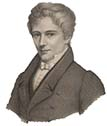
\includegraphics[width=0.13\textwidth]{abel.jpg}
 \end{enumerate}
 \vspace*{50pt}
  \end{definition}

  Most groups are not abelian. Example: in $GL_2()$, we have:

\[\begin{pmatrix}
1 & -1 \\ 0 & 2
\end{pmatrix}
\begin{pmatrix}
0 & 1 \\ 1 & 0
\end{pmatrix}
= 
\begin{pmatrix}
-1 & 1\\ 2 & 0
\end{pmatrix}\]

But 
\[
\begin{pmatrix}
0 & 1 \\ 1 & 0
\end{pmatrix}
\begin{pmatrix}
1 & -1 \\ 0 & 2
\end{pmatrix}
=
\begin{pmatrix}
0 & 2 \\ 1 & -1
\end{pmatrix}\]

So $\left(\begin{smallmatrix}
0 & 1\\ 1 & 0
\end{smallmatrix}\right)
$ and $\left(\begin{smallmatrix}
1 & -1\\ 0 & 2
\end{smallmatrix}\right)
$ do not commute, so $GL_2(\mathbb{R})$ is not abelian.\\


But many of the groups we have seen so far are abelian.\\

Examples: $(\Z,+), (F,+), (F\backslash\{0\},\times), GL_1(F), (\{1,-1,i,-i\},\times) $ are all abelian.\\

\begin{definition} Let $X$ be a set. A function $f : X \to X$ is a \emph{permutation}\index{Permutation} of $X$ if it is a bijection. (Injective + surjective). 	
\end{definition}\vspace*{10pt}

\begin{examples} \begin{enumerate}
 \item $X = \{1,2,3,4\}$. $f : 1 \mapsto 2, ~2 \mapsto 3,~ 3\mapsto 4,~ 4 \mapsto 1 $ is a permutation.
 \item $X = \Z, f: n \mapsto n+3$ is a permutation.
 \item $X = \Z$, $f: n \mapsto 3n$ is \emph{not} a permutation, (not surjective).
 \end{enumerate}
 \end{examples}\vspace*{10pt}
 
\noindent \textbf{Notation for permutations} (First attempt.)    \lecturemarker{14}{13/02} 
\\

Assume that $X = \{1,\dots,n\}$. Let $f: X \to X$ be a permutation. We can write $f$ as a matrix with two rows: \[
\begin{pmatrix}
1 & 2 & \dots & n\\ f(1) & f(2) & \dots & f(n)	
\end{pmatrix}\]

is called \emph{two-row rotation.}\\

Examples: if $f : 1 \mapsto 2, ~2 \mapsto 3,~ 3\mapsto 4,~ 4 \mapsto 1 $, we can write $f$ as $\left(\begin{smallmatrix}
1 & 2 & 3 & 4\\ 2 & 3 & 4 & 1	
\end{smallmatrix}\right)$. If $g$ is $\left(\begin{smallmatrix}
1 & 2 & 3 & 4\\ 3 & 1 & 2 & 4	
\end{smallmatrix}\right)$, then $g: 1 \mapsto 3,~2 \mapsto 1, 3\mapsto 2, 4\mapsto 4$.\\


Let $f$ and $g$ be permutations of a set $X$. We define the \emph{composition}\index{Composition}, $f \circ g$ by $f \circ g(x) = f(g(x))$ for all $x \in X$. For example, if $f$ and $g$ are as in the example above, we have $f \circ g(1) = 4, f\circ g(2) = 2, f\circ g(3) = 3, f \circ g(4) = 1$. So $f\circ g =
 \left(\begin{smallmatrix}
1 & 2 & 3 & 4\\ 4 & 2 & 3 & 1	
\end{smallmatrix}\right)$.\\


\begin{proposition} Let $X$ be any set. Let $S$ be the set of all permutations of $X$. Let $\circ$ be the composition operation as above. Then $(S,\circ)$ is a group, called the \emph{symmetric group}\index{Symmetric Group} on $X$, written Sym$(X)$.	
\end{proposition}


\begin{proof}
We first check that $\circ$ is a binary operation on $S$. Certainly if $f: X \to X$ and $g: X \to X$, then $f \circ g: X \to X$. The composition of two bijections is a bijection. So if $f,g  \in S$, then $f\circ g \in S$.\\

Now the group axioms:\begin{enumerate}
\item \textsc{Associativity:} If $x \in X$, and $f,g,h \in S$, then $(f \circ g) \circ h(x) = (f\circ g)(h(x)) = f(g(h(x))) = f(g \circ h(x)) = f \circ(g \circ h(x))$. Since they agree on all $x \in X$, we have $(f \circ g) \circ h = f \circ(g \circ h)).$
\item \textsc{Identity:} Let $e$ be the permutation defined by $e(x) = x$ for all $x \in X$. Then we have $e\circ f(x) = f(x) = f \circ e(x)$ for all $f\in S$. So $e\circ f = f \circ e = f$.
\item \textsc{Inverses:} Bijections have inverses.
\end{enumerate} \vspace*{-10pt}
\end{proof}

\noindent \textbf{Further notation:} We almost always write symmetric groups multiplicatively. So write $fg$ for $f\circ g$, and so on.\\
 When $X = \{1,\dots,n\}$, we write $S_n$ for the Sym$(X)$.\\
 
 
\begin{examples} $S_1$ = Sym$(\{1\}) = \{e\} = (	1,1)^T$.\\
 
 $S_2 = $ Sym$\{1,2\}$ = $\{e, \left(\begin{smallmatrix}
1 & 2 \\ 2 & 1	
\end{smallmatrix}\right)\}$\\

$S_3 = $ Sym$\{1,2,3\}$ = $\{e, \left(\begin{smallmatrix}
1 & 2 & 3 \\ 2 & 3 & 1	
\end{smallmatrix}\right),\left(\begin{smallmatrix}
1 & 2 & 3 \\ 3 & 1 & 2
\end{smallmatrix}\right),\left(\begin{smallmatrix}
1 & 2 & 3 \\ 2 & 1 & 3	
\end{smallmatrix}\right),\left(\begin{smallmatrix}
1 & 2 & 3 \\ 3 & 2 & 1
\end{smallmatrix}\right),
\left(\begin{smallmatrix}
1 & 2 & 3 \\ 1 & 3 & 2
\end{smallmatrix}\right)
\}$.

We have $|S_1| = 1, |S_2| = 2, |S_3| = 6$
\end{examples}\vspace*{10pt}

\begin{proposition} The group $S_n$ has order $n!$	
\end{proposition}

\begin{proof}
	By induction. Inductive hypothesis. if $X$ and $Y$ are the two set of size $n$, then the number of bijections form $X$ to $Y$ is $n!$. (This gives us the result by taking $Y=X$.)\\
	
	Base case $n=1$ is obvious.\\
	Inductive step: Suppose the result is true for $n$:\\
	
	Let $|X| = |Y| = n+1$. Take $x \in X$, $y \in Y$. The number of bijections $f: X \to Y$ such that $f(x) = y$ is equal to the number of bijections $X\backslash\{x\} \to Y\backslash\{y\}$, which is $n!$ by the inductive hypothesis. So the total number of bijections $X \to Y$ is $(n+1)n! =  (n+1)!$.
\end{proof}


\noindent \textbf{The Group Table.} Let $G$ be a finite group. We can record the multiplication (binary operation) in $G$ in a table called the \emph{Group Table} or \emph{Cayley Table}\index{Group Table} of $G$. If $G =\{a,b,c,\dots\}$, write:
 \[
    \begin{tabular}{>{$}l<{$}|*{4}{>{$}l<{$}}}
    ~  & a   & b   & c & \dots  \\
    \hline\vrule height 12pt width 0pt
    a   & aa  & ab    & ac & ~  \\
    b   & ba   & bb & bc  & \dots   \\
    c & ca & cb    & cc  &~   \\
    \vdots & ~ & \vdots & ~ & ~
    \end{tabular} 
\]

\begin{example} Let $G = S_3$\\

 Write $a = \left(\begin{smallmatrix}
1 & 2 & 3 \\ 2 & 3 & 1	
\end{smallmatrix}\right).$ Then $a^2 = \left(\begin{smallmatrix}
1 & 2 & 3 \\ 3 & 1 & 2
\end{smallmatrix}\right),$ and $a^3 = e$.\\

Write $b = \left(\begin{smallmatrix}
1 & 2 & 3 \\ 1 & 3 & 2	
\end{smallmatrix}\right).$ Then $b^2= \left(\begin{smallmatrix}
1 & 2 & 3 \\ 2 & 1 & 3
\end{smallmatrix}\right),~ a^2b
\left(\begin{smallmatrix}
1 & 2 & 3 \\ 3 & 1 & 2
\end{smallmatrix}\right)$.\\

So $S_3 = \{e, a, a^2, b, ab, a^2b\}$. To work out the group table, it is helpful to check: $b^2 = e, ba = a^2b, ba^2 = ab$. Now it is easy to write down:

 \[
    \begin{tabular}{>{$}l<{$}|*{6}{>{$}l<{$}}}
    ~  & e   & a   & a^2 & b & ab & a^2b  \\
    \hline\vrule height 12pt width 0pt
    e  & e  & a & a^2    & b & ab & a^2b \\
    a   & a & a^2 & e & ab & a^2b & b\\
    a^2 & a^2 & e & a & a^2b  & b  & ab \\
    b & b & a^2b & ab & e & a^2 & a\\
    ab & ab &  b & a^2b & a & e & a^2\\
    a^2b & a^2b & ab & b & a^2 & a & e
    \end{tabular} 
\]

Notice that every element of the group appears exactly once in each row and each column. (This follows from left and right cancellation laws.)
\end{example}\vspace*{10pt}


\subsektion{Subgroups}


\begin{definition} Let $(G,*)$ be a group. A \emph{subgroup}\index{Subgroup} of $G$ is a subset of $G$ which is itself a group under the operation $*$.	
\end{definition}\vspace*{10pt}


\begin{examples}\begin{enumerate}
 \item[(i)] $(\Z,+)$ is a subgroup of $(\Q,+)$. Both are subgroups of $(\mathbb{R},+)$. All are subgroups of $(\C,+)$. But $(\mathbb{N},+)$
 is not a subgroup of any - it has no inverses.
 \item[(ii)] $(\mathbb{R} \backslash\{0\},\times)$ is not a subgroup of $(\mathbb{R},+)$. The group operation is different.
 \item[(iii)] $\{e\}$ is a subgroup of any group (where $e$ is the identity element). The \emph{trivial} subgroup.
 \item[(iv)] Every group is a subgroup of itself.
  \end{enumerate}
  \end{examples}\vspace*{10pt}

\emph{Recall:} \lecturemarker{15}{17/02} 
a subgroup of a group $G$ is a subset of $G$ which is a group under the same operation as $G$.\\

\begin{proposition} (Subgroup Criteria) Let $G$ be a group. We write $G$ multiplicatively. Let $H \subseteq G$ be a subset. Then $H$ is a subgroup if and only if the following conditions hold:\begin{enumerate}
\item $e \in H$, where $e$ is the identity of $G$.
\item If $a,b \in H$, then $ab \in H$, for all $a,b \in G$.
\item If $a \in H$, then $a^{-1} \in H$, where $a^{-1}$ is the inverse of $a$ in $G$.	
\end{enumerate}
\end{proposition}

\begin{proof}
\textbf{``if''}. Condition (2) says that the binary operation on $G$ restricts to a binary operation on $H$. Since the operation is associative on $G$, it is also associative on $H$. Condition (1) gives us an identity, and Condition (3) gives inverses. So if (1),(2),(3) hold then $H$ is a subgroup.\\

\textbf{``only if''}. Certainly (2) must hold if $H$ is a subgroup, since we need the binary operation on $G$ to restrict to a binary operation on $H$. If $H$ is a subgroup, then $H$ has an identity, $e_H$. Write $e_G$ for the identity of $G$. Then $e_Ge_H = e_H$, and also $e_He_H = e_H$. Now $e_G = e_H$, by right cancellation. So $e_G \in H$, and so (1) holds.\\

Let $a \in H$. Let $b$ be the inverse of $a$ in $G$, and let $c$ be the inverse of $a$ in $H$. $ab = e_G = e_H = ac$. So $b=c$ by left cancellation. So $b \in H$, and so (3) holds.
\end{proof}\vspace*{10pt}

\begin{example} Let $G = GL_2()$. For $n \in \Z$, define $u_n = \left(\begin{smallmatrix}
1 & n \\ 0 & 1	
\end{smallmatrix}\right)
$, so $u_n \in G$, for all $n \in \Z$. Define $U = \{u_n ~:~ n \in \Z\}$. Then $U$ is a subgroup of $G$. Check the subgroup criteria: \begin{enumerate}
 \item $e_G = I = u_0 \in U$
 \item $u_mu_n = \left(\begin{smallmatrix}
1 & m \\ 0 & 1	
\end{smallmatrix}\right)\left(\begin{smallmatrix}
1 & n \\ 0 & 1	
\end{smallmatrix}\right) = 
\left(\begin{smallmatrix}
1 & m+n \\ 0 & 1	
\end{smallmatrix}\right) = u_{m+n} \in U$	
\item From (1) and (2), we see that $u_m^{-1} = u_{-m}$, so $u_{m}^{-1} \in U$. So $U$ is a subgroup.
 \end{enumerate} 
 \end{example}
 
\noindent \textbf{Notation:} If $H$ is a subgroup of $G$, we write $H \leq G$. (We can write $H < G$ if $H \neq G$).\\

\noindent \textbf{Powers in groups:} Let $G$ be a a group written multiplicatively. Let $g \in G$. We can write $g^1 = g, ~ g^2 = gg,~ g^3 = ggg$, and so on. We also write $g^{0} = e$, and $g^{-n} = (g^{-1})^n$. So now $g^n$ is defined for all $n \in \Z$.\\

\begin{proposition}\begin{itemize}
 \item[(a)] $(g^n)^{-1} = g^{-n}$.
 \item[(b)] $g^mg^n = g^{m+n}$.
 \item[(c)] $(g^m)^n = g^{mn}$.	
 \end{itemize}
 \end{proposition}
 
 \emph{Proof omitted.}\\
 
 \noindent \textit{Caution:} It is not generally true that $a^nb^n = (ab)^n$. (Though true for Abelian Group)\\
 
\subsektion{Cyclic Subgroups} 
\begin{proposition} Let $G$ be a group, and let $g \in G$. Define $\langle g\rangle  = \{g^n : n \in \Z\}$. Then $\langle g\rangle $  is a subgroup of $G$.	
\end{proposition}

 \begin{proof}
 	Check subgroup criteria: \begin{enumerate}
 \item $g^{0} = e$
 \item $g^mg^n = g^{m+n}$
 \item $(g^n)^{-1} = g^{-n}$ \qedhere 
 \end{enumerate}\end{proof}\vspace*{10pt}
 

\begin{definition} The subgroup $\langle g \rangle$ is the \emph{cyclic subgroup}\index{Cyclic Subgroup} generated by $g$.
	
\end{definition}\vspace*{10pt}

\begin{examples} \begin{enumerate}
 \item $U = \{u_n = \left(\begin{smallmatrix}
1 & n \\ 0 & 1	
\end{smallmatrix}\right) ~:~ n \in \Z
\}$	is $\langle u_1 \rangle $. (Easy induction to show that $\left(\begin{smallmatrix}
1 & 1 \\ 0 & 1	
\end{smallmatrix}\right)^n = \left(\begin{smallmatrix}
1 & n \\ 0 & 1	
\end{smallmatrix}\right)$ for all $n \in Z$)
\item In $(\Z,+),$ what is $\langle 3 \rangle $?\\
Note that we write this group additively, write $ng$ instead of $g^n$. So $\langle 3 \rangle = \{n.3 ~:~ n \in \Z\}$. So $\langle 3 \rangle$ contains precisely all multiples of 3.
\item $G = S_3$. What are the cyclic subgroups? From the group table we can easily calculate:\\\vspace{5pt}
$\langle e \rangle = \{e\}$\\ \vspace{5pt}
$\langle a \rangle = \{e,a,a^2\}$, since $a^3 = e$.\\\vspace{5pt}
$\langle a^2 \rangle = \{e,a,a^2\}$\\\vspace{5pt}
$\langle b\rangle = \{e,b\}$ since $b^2 = e$\\\vspace{5pt}
$\langle ab \rangle = \{e,ab\}$, since $(ab)^2 = e$\\\vspace{5pt}
$\langle a^2b \rangle = \{e,a^2b\}$, since $(a^2b)^2 = e$\\
 \end{enumerate}
 \end{examples}\vspace*{10pt}
 
\textit{Recall:}  \lecturemarker{16}{18 /02} 
$\langle g \rangle = \{g^n : n \in \Z\}$\\

\begin{definition} A group is \emph{cyclic}\index{Cyclic Group} if $G = \langle g \rangle $ for some $g \in G$. In this case $g$ is a \emph{generator}\index{Generator} for $G$.
	
\end{definition}\vspace*{10pt}

\begin{examples}\begin{enumerate}
\item[(i)] $(\Z,+)$	is cyclic, since $\Z = \langle 1 \rangle$. Another generator is $-1$. There are no other generators.
\item[(ii)] $\{1,-1,i,-i\}$ is cyclic, since it is equal to $\langle i \rangle $, and $\langle -i \rangle$. So $i$ and $-i$ are generators. 1 and $-1$ are not.
\item[(iii)] Let $\Omega_n = \{$ complex $n$th roots of unity $\}$, under complex multiplication. Let $w = e^{2\pi i/n}$. Then $\langle w \rangle = \{e^{2\pi i k/n} : k \in \Z\} = \Omega_n$. So $\Omega_n$ is a a group - a cyclic subgroup of $\C$.

Since $|\Omega_n| = n$, it follows that there exists a group of order $n$ for $n \in \mathbb{N}$.

\item[(iv)] $S_3$ is \emph{not} cyclic. We have calculated all of its cyclic subgroups (Example 76, 3), and none of them were equal to $S_3$.
 \end{enumerate}
 \end{examples}
 
 \subsektion{The Order of a Group Element}
 
\begin{definition} Let $G$ be a group, and $g \in G$. The \emph{order}\index{Order of Element} of $g$ is the least positive integer $k$, such that $g^k = e$, if such an integer exists. Otherwise $g$ has infinite order. Write ord$(g)$ or o$(g)$ for the order of $g$. Write ord$(g) = \infty$ if $g$ has infinite order.	
\end{definition}\vspace*{10pt}

\begin{examples}\begin{enumerate}
 \item[(i)] In any group $G$, the identity $e$ has order 1. No other element has order 1. (If $g^1 = e$ then $g = e$.)
 
 \item[(ii)] Let $G = S_3$ Let $a  = \left(\begin{smallmatrix}
1 & 2 & 3 \\ 2 & 3 & 1	
\end{smallmatrix}\right)$. Then $a^1 \neq e$, $a^2 = \left(\begin{smallmatrix}
1 & 2 & 3 \\ 3 & 1 & 2 	
\end{smallmatrix}\right) \neq e$. But $a^3 = e$. So ord $(a)$ = 3.

 Let $b = \left(\begin{smallmatrix}
1 & 2 & 3 \\ 1 & 3 & 2	
\end{smallmatrix}\right).$ Then $b \neq e$, but $b^2 = e$. So ord$(b)$ = 2. Can also check that ord$(a^2)$ = 3, ord$(ab)$ = 2, ord$(a^2b)$ = 2.


\item[(iii)] Let $G = (\Z,+)$. We know that ord$(0)$ = 1. Suppose $n \neq 0$. Then since $\underbrace{n + n + \dots n}_{k} = kn \neq 0$ for any positive integer $k$. We must have ord $(n)$ = $\infty$.
\item[(iv)] $G = GL_2(\C)$. Let $A = \left(\begin{smallmatrix}
i & 0 \\ 0 & e^{2 \pi i/3} 	
\end{smallmatrix}\right)$. \emph{What is the order of $A$?}\\

We see that for $k \in \Z$ we have $A^k = \left(\begin{smallmatrix}
i^k & 0 \\ 0 & e^{2\pi ik/n}	
\end{smallmatrix}\right)
$, which is equal to $\left(\begin{smallmatrix}
1 & 0 \\ 0 & 1	
\end{smallmatrix}\right)$ if and only if $i^k = 1$ and $e^{2 \pi ik/n} = 1$.\\

 Now $i^k = 1$ if and only if $4 ~|~ k$, and $e^{2\pi ik/n} = 1$ if and only if $3 ~|~ k$. So $A^k = I$ if and only if $12 ~|~ k$. Since the smallest positive integer divisible by 12 is 12, we have ord($A$) = 12.
 \end{enumerate}
 \end{examples}\vspace*{10pt}
 
\begin{proposition} If $G$ is a group and $g \in G$, then $|\langle g \rangle| = $ ord $(g)$. ($\langle g \rangle$ is infinite $\iff$ ord $(g) = \infty$).	
\end{proposition}

 
 \begin{proof}
 Suppose first that ord$(g) = \infty$. So $g^k \neq e$ for any $k \in \mathbb{N}$. We claim that if $m \neq n \in \Z$, then $g^m \neq g^n$. Suppose w.l.o.g. that $n > m$. Let $k = n-m$. Then $k \in \mathbb{N}$. Now $g^n = g^{m+k} = g^mg^k$. If $g^m = g^n$, then $g^m = g^mg^k$, and so $g^k = e$ by left cancellation. But this is a contradiction, and this proves the claim.\\
 Now we have $g^0,g^1,g^2,g^3,\dots$ are all distinct elements of $\langle g \rangle$, and so $\langle g \rangle$ is infinite.\\
 
 Now suppose that ord$(g) = k \in \mathbb{N}$. I claim that $\langle g \rangle = \{g^0,g^1,\dots,g^{k-1}\}$, and that the elements $g^0,\dots,g^{k-1}$, are distinct. (So $|\langle g \rangle| = k$). We use the fact that $n \in \Z$ can be written as $pk + q$, where  $p,q \in \Z$ and $0 \leq q < k$. So $g^n = g^{pk+q} = (g^k)^pg^q = e^pg^q = g^q$. But $g^q$ is one of the elements $g^0,\dots,g^{k-1}$, and so $\langle g \rangle = \{g^0,\dots,g^{k-1}\}$.\\
 
  Suppose $g^i = g^j$, where $0 \leq i < j \leq k-1$. Let $l = j-i.$ Then $g^i = g^j = g^{i + l}$, and so $g^l = e$ by left cancellation. But $l$ is a positive integer less than $k$, so this contradicts the assumption that ord$(g)$ = $k$. This proves the claim.
 \end{proof}


We have seen Proposition 81 illustrated in several examples already.\\

\begin{examples} \begin{enumerate}
 \item[(i)] Comparing the list of cyclic subgroups of $S_3$ with the list of the orders of elements, we saw that ord$(g) = |\langle g \rangle|$ in each case.
 \item[(ii)] In the case $G = (\Z,+)$, we saw that $\langle 3 \rangle = 3\Z = \{3k : k \in \Z\}$. So $|\langle 3 \rangle| = \infty$, and we have also seen that ord$(3) = \infty$.
 \item[(iii)] If $w = e^{2\pi i/n}$, then clearly ord$(w) = n$. And $\langle w \rangle = \Omega_n$ has order $n$ too.	
 \end{enumerate}
\end{examples}\vspace*{10pt}

\subsektion{Cycles}
 
Let \lecturemarker{17}{20/02} 
 $f = \left(\begin{smallmatrix}
1 & 2 & 3 & 4 & 5 & 6 & 7 & 8 \\
4 & 5 & 6 & 3 & 2 & 7 & 1 & 8	
\end{smallmatrix}\right)$. Looking at the successive images of 1 under the permutation $f$, we get back to 1 again after 5 steps via 4,3,6,7.


\begin{center}   
 \begin{tikzpicture}
 $f$~~
\node (P0) at (90:1.4cm) {$1$};
\node (P1) at (90+72:1.4cm) {$7$} ;
\node (P2) at (90+2*72:1.4cm) {$6$};
\node (P3) at (90+3*72:1.4cm) {$3$};
\node (P4) at (90+4*72:1.4cm) {$4$};
\draw
(P0) edge[<-|,>=angle 90] node[left] {} (P1)
(P1) edge[<-|,>=angle 90] node[left] {} (P2)
(P2) edge[<-|,>=angle 90] node[above] {} (P3)
(P4) edge[|->,>=angle 90] node[right] {} (P3)
(P0) edge[|->,>=angle 90] node[right] {} (P4);
\end{tikzpicture}
\end{center}


We say that 1,4,3,6,7 forms a 5-cycle of $f$. Write $(1 ~4~ 3 ~6~ 7)$ for this cycle.\\

Similarly:\begin{tikzcd}
2\arrow[mapsto,bend left]{r} \arrow[mapsfrom,bend right]{r}{f}&5
\end{tikzcd} is a 2-cycle, written $(2~5)$.\\

 Finally 8 is a fixed point or 1-cycle of $f$. We can write $(8)$ if we like $-$ but usually we do not write out 1-cycles.\\
 
 
 We can think of cycles as permutations in their own right. Take everything outside the cycle to be fixed.\\
 
  So $(1~4~3~6~7)$ is the permutation: $\left(\begin{smallmatrix}
1 & 2 & 3 & 4 & 5 & 6 & 7 & 8\\
4 & 2 & 6 & 3 & 5 & 7 & 1 & 8 	
\end{smallmatrix}\right)$.\\

 And $(2~5)$ is the permutation: $\left(\begin{smallmatrix}
1 & 2 & 3 & 4 & 5 & 6 & 7 & 8\\
1 & 5 & 3 & 4 & 2 & 6 & 7 & 8 	
\end{smallmatrix}\right)$. \\

And $(8)$ represents the identity permutation.\\


Notice that $f =  (1~4~3~6~7)(2~5)$ (where the cycles are multiplied by composition, as elements of $S_8)$. So we have factorised $f$ into cycles. These cycles have no common points $-$ they are disjoint. This is the \emph{disjoint cycle notation}\index{Disjoint Cycles} for $f$.\\


\begin{method}To calculate the disjoint cycle notation for a permutation $f \in S_n$.\begin{enumerate}

\item[Step 1.] Pick the least element $i \in \{1,\dots,n\}$ which  we haven't used yet. (Initially, we choose $i=1$.) Open a new cycle with $i$. 

\item[Step 2.] Continue the cycle with successive images of $i$ under $f$ until we get back to $i$ again. Then close the cycle.

\item[Step 3.] If all $i \in \{1,\dots,n\}$ have appeared, then stop. Otherwise go back to Step 1.

\end{enumerate}
\end{method}\vspace*{10pt}

\begin{examples}$f = \begin{pmatrix}
1 & 2 & 3 & 4 & 5 & 6 & 7 & 8 & 9 & 10\\
3 & 6 & 1 & 7 & 5 & 8 & 2 & 4 & 10 & 9	
\end{pmatrix}$. \\

Open a cycle with 1. Continue the cycle with $f(1) = 3$. Since $f(3)$ is 1 again, close the cycle. $(1~3)$. \\

Now open a new cycle with 2. Continue it with 6,8,4,7. Since $f(7) = 2$, we then close the cycle. $(2~6~8~4~7)$. \\

Start a cycle with 5. But 5 is a fixed-point of $f$, so close the cycle immediately. $(5)$.\\

Finally, start a cycle with 9. Continue it with $f(9) = 10$. But $f(10) = 9$, so close the cycle. $(9~10)$.\\

Now all points have appeared, so we stop. So the disjoint cycle notation for $f$ is $f = (1~3)(2~6~8~4~7)(5)(9~10)$. We usually omit 1-cycles. So $f = (1~3)(2~6~8~4~7)(9~10)$.
\end{examples}\vspace*{10pt}

\begin{proposition} Method 83 always works. Every permutation in $S_n$ can be written as a product of disjoint cycles.	
\end{proposition}


\begin{proof}
	First we show that whenever we open a new cycle at Step 1, we are able to close it at Step 2. (We always get back to the starting point eventually.)\\
	
	Suppose that $x$ is the starting point. Since $n$ is finite, the points $x, f(x), f^2(x),\dots$ cannot be all distinct. So there must exist some least $k$ such that $f^k(x) = f^j(x)$, for some $j < k$. Suppose that $j \neq 0$. Then $f^{-1}f^k(x) = f^{-1}f^j(x),$ and so $f^{k-1}(x) = f^{j-1}(x)$.\\
	
	 But this contradicts the assumption that $k$ was the \emph{least} to give a repeat. So by contradiction, we must have $j = 0$. So $f^k(x) = f^0(x) = x$. So the first repeated term in the cycle is $x$ itself, and we close the cycle at that point.\\
	 
	 Next we check that the cycles arising from Method 83. are disjoint. Let $c$ and $d$ be two cycles. Suppose that $c$ starts with $x$ and $d$ starts with $y$. Suppose that $c$ was constructed first. Then $y$ cannot be in the cycle $c$ (since otherwise we would not have used it to start a new cycle.)\\
	 
	 Suppose $z$ is in both $c$ and $d$. So $z = f^i(x) = f^j(y)$ for some $i,j$. But now $f^{i-j}(x) = y$ This implies that $y$ is in the cycle $c$, which is a contradiction. Hence $c$ and $d$ are disjoint.
\end{proof}\vspace*{10pt}


\noindent \textbf{Multiplication.} To multiply permutations given in disjoint cycle notation, recall that $fg = f \circ g,$ so $fg(x) = f(g(x))$. Now use Method 83 to get the disjoint cycle notation of $fg$. \\

\textit{Example:} $f = (1~3~5)(2~4~6)$, $g = (1~2~3~4)(5~6) \in S_6$. Calculate $fg: 1 \mapsto 4 \mapsto 3 \mapsto 6 \mapsto 1\quad $ $2\mapsto 5 \mapsto 2$. Hence $fg = (1~4~3~6)(2~5)$.\\
 
 
 \noindent \textbf{Inverses.} These are very easy~ Just write the cycles backwards.\\ 
 
 If $f = (1~3~5)(2~4~6)$, then $f^{-1} = (5~3~1)(6~4~2) = (1~5~3)(2~6~4)$.\\
  
 \noindent \textbf{Non-uniqueness.} \begin{enumerate}
 \item[i.] Order of the cycles doesn't matter.	
 \item[ii.] The choice of starting point in each cycle doesn't matter.
 \item[iii.] We can include or exclude 1-cycles.
 \end{enumerate}~\\
 
\begin{example}\lecturemarker{18}{24/02} 
 In disjoint cycle notation, the group table for $S_3$ from Example 68 becomes:


 \[
    \begin{tabular}{>{$}l<{$}|*{6}{>{$}l<{$}}}
    ~  & e   & (123)   & (132) & (23) & (12) & (13)  \\
    \hline\vrule height 12pt width 0pt
    e  & e   & (123)   & (132) & (23) & (12) & (13) \\
    (123)   & (123) & (132) & e & (12) & (13)& (23)\\
    (132) & (132) & e & (123) & (13) & (23) & (12) \\
    (23) & (23) & (13) & (12) & e & (132) & (123)\\
    (12) & (12) &  (23) & (13) & (123) & e & (132)\\
    (13) & (132) & (12) & (23) & (132)& (123) & e
    \end{tabular} 
\]
\end{example}
\vspace*{10pt}

\begin{remark} Disjoint cycles commmute. (If cycles $c_1$ and $c_2$ have no points in common, then $c_1c_2 = c_2c_1$). Example: $(12)(345) = (345)(12)$.\\

 Cycles which are not disjoint don't usually commute. Example: $(12)(13) = (132)$. $(13)(12) = (123)$.
 \end{remark}\vspace*{10pt}
 

\begin{definition} The \emph{cycle shape}\index{Cycle Shape} of a permutation is the sequence of cycle lengths in descending order of size when the permutation is written in disjoint cycle notation. We include $1-$cycles.	
\end{definition}\vspace*{10pt}

Example: $f = (12)(3)(456)(7)(89) \in S_9$ then $f$ has cycle shape $(3,2,2,1,1)$. We abbreviate this to $(3,2^2,1^2).$ The identity of $S_9$ has cycle shape $(1,1,1,1,1,1,1,1,1),$ or  $(1^9)$.\\


\begin{examples}What are the cycle shapes in $S_4$, and how many elements are there of each shape?\\

Cycle shapes are given by weakly decreasing sequences of positive integers adding up to 4. There are $(4)$, $(3,1)$, $(2^2)$, $(2,1^2)$ and $(1^4)$. (These are the \emph{partitions} of the integer 4). How many of each type? \begin{itemize}
 \item[$(4)$:] May start the cycle at 1. There are 3 choices for $f(1)$. Then there are 2 choices for $f^2(1)$. This determines the cycle. So 6 possible 4-cycles. (These are $(1234),~(1243),~(1324),~(1342),~(1423),(1432)$.)
 \item[$(3,1)$:] There are 4 choices for the fixed-point (or 1-cycle).  Once the fixed point is chosen, there are 2 choices for the 3-cycle. So there are 8 possible permutations with this shape.
 \item[$(2^2)$:] 1 is in a 2-cycle, and there are 3 choices for the other point in that cycle. This determines the permutation. So there are only 3 permutations with this shape. These are $(12)(34),~(13)(24),~(14)(23)$.
 \item[$(2,1^2)$:] There are $\left(\begin{smallmatrix}
4 \\ 2	
\end{smallmatrix}\right)$ ways of choosing the two fixed points. This determines the permutations. So there are 6 permutations.
\item[$(1^4)$:] Only the identity has this shape. 
 \end{itemize}
 
 Check: we have $6 + 8 + 3 + 6 + 1 = 24 = |S_4|$.
\end{examples}


 \subsektion{Order of a Permutation}
 
\begin{proposition} Let $G$ be a group, and let $g \in G$. Suppose ord$(g) = d$. Then for all $k\in \Z$, we have $g^k = e \iff d~|~k $.	
\end{proposition}

 
 \begin{proof}
 By Euclid's Lemma, we can write $k = xd + y,$ where $x,y \in \Z$ and $0 \leq y < d$. Now $g^k = g^{xd + y} = (g^d)^xg^y = e^xg^y = g^y$. But $y < d$, and so we have $g^y = e \iff y =0 \iff d~|~k$.
 \end{proof}\vspace*{10pt}
 
\begin{proposition}Let $G$ be a group, and let $a,b\in G$ be elements such that $ab = ba$. Then: \begin{enumerate}
 \item $a^{-1}b = ba^{-1}$
 \item $a^ib^j = b^ja^i$, for $i,j \in \Z$.
 \item $(ab)^k = a^kb^k$, for $k \in \Z.$	
 \end{enumerate}
 \end{proposition}
 
 \begin{proof}~\\ 
 
 1. We have $ab = ba.$ So $a^{-1}(ab)a^{-1} = a^{-1}(ba)a^{-1}$. Hence $ba^{-1} =  a^{-1}b$.\\
 
 2. If $j < 0$, then replace $b$ with $b^{-1}$. We know $ab^{-1} = b^{-1}a$ by 1. In this way, we may assume $j \geq 0$. Now by induction on $j$. [left as exercise.]\\
 
 3. If $k < 0$, then write $d = a^{-1},~c = b^{-1}$. Then $(ab)^{-1} = cd$, and so $(ab)^k = (cd)^{-k}$. In this way we may assume $k \geq 0$. Now work by induction on $k$. [left as exercise.]
 \end{proof}\vspace*{10pt}

 
 
\begin{proposition} Let $f$ be a permutation with cycle shape $(r_1,r_2,\dots,r_k)$. Then ord$(f) =$ lcm$(r_1,r_2,\dots,r_k)$.	
\end{proposition}


 \begin{proof} 

Write  \lecturemarker{19}{25/02} $f = c_1c_2\dots c_k$, where $c_i$ has length $r_i$ for all $i$, and the cycles $c_i$ are disjoint from one another.\\

Recall \textit{Remark 87}: disjoint cycles commute. So $c_ic_j = c_jc_i$, for all $i,j$. Let $t \in \Z$. \textbf{Claim:} $f^t = c_1^tc_2^t\dots c_k^t$. 
\begin{proof}[Proof of Claim] First observe that $f = c_1,\dots,c_{k-1}c_k = c_kc_1,\dots,c_{k-1}$, since $c_k$ commutes with all of the other cycles. So $c_k$ commutes with $c_1\dots c_{k-1}$. So by Prop 91.3, we have $f^t = ((c_1\dots c_{k-1})c_k)^t =(c_1\dots c_{k-1})^t  c_k^t $. Now an easy induction on $k$ gives that $f^t = c_1^tc_2^t\dots c_k^t$, as required.
\end{proof}

Continuing the proof of Prop 92, we see that $f^t = e \iff c_i^t = e$, for all $i$. But $c_i^t = e$ if and only if $r_i ~|~ t$. So $f^t = e \iff r_i ~|~ t$, for all $i \iff t$ is divisible by lcm$(r_1,r_2,\dots,r_k)$.\\

So ord$(f)$ is the last positive integer divisible by lcm$(r_1,\dots,r_k)$, which is lcm$(r_1,\dots,r_k)$ itself.
 \end{proof}\vspace*{10pt}
 
\begin{examples} \begin{enumerate}
 \item[(i)] ord$((12)(3456))$ = lcm$(2,4) = 4.$
 \item[(ii)] ord$(13)(3456)) \neq 4 -$ the cycles are not disjoint. We calculate $(13)(3456) = (13456)$, which has order 5.
 \item[(iii)] Clearly 1-cycles never affect the order of a permutation.
 \item[(iv)] Suppose we have a pack of 8 cards. We shuffle them by cutting the pack into 2 equal parts, and then interleaving the parts. \vspace*{-5pt}
 
 We get the permutation $\left(\begin{smallmatrix}
	1 & 2 & 3 & 4 & 5 & 6 & 7 & 8 \\ 1 & 5 & 2 & 6 & 3 & 7  & 4 & 8
\end{smallmatrix}\right).$ In disjoint cycle form, this is $(253)(467)$, which has order 3. So if we repeat our shuffle three times, the pack is back in its original order.
\end{enumerate}
\end{examples}\vspace*{10pt}

\textit{Exercise: How many shuffles do you need for a full pack of 52 cards to be shuffled back to its original order?}
\vspace*{10pt}
 
 \subsektion{Lagrange's Theorem}
 
 
\begin{theorem}[Lagrange's Theorem]\index{Lagrange's Theorem|idxbf}  Let $G$ be a finite group. Let $H$ be a subgroup of $G$. Then $|H|$ divides $|G|$.	
\end{theorem}\vspace*{10pt}

 
\begin{examples}\begin{enumerate}
 \item $|S_3| = 6$. We have seen that the cyclic subgroups of $S_3$ have orders $1,2,3$. There are no other subgroups, except $S_3$ itself.
 \item $G = \{1,-1,i,-i\}$, order 4. The subgroups of $G$ are $\{1\},\{1,-1\}$, and $G$, with orders $ 1,2,4.$
 \item Let $C_n = \langle w \rangle \leq \C \backslash\{0\}$, where $w = e^{2\pi i/n}$. If $d$ divides $n$, then $w^{n/d} = e^{2\pi i/d}$, which has order $d$. So $\langle w^{n/d} \rangle$ is a subgroup of $C_n$ with order $d$. In fact all of the subgroups of $C_n$ have this form, for some $d$.
 \end{enumerate}
 \end{examples}\vspace*{10pt}

\noindent \textit{Remark.} Although it is true for the elementary groups above, it is not true in general that a group $G$ has a subgroup of order $d$ for every divisor.\\
 Example: $S_5$ has order 120, but has no subgroup of order $15,30,40$.\\
 
 
\begin{corollary} (to Lagrange's Theorem) If $G$ is a finite group, and $g \in G$, then ord$(g)$ divides $G$.	
\end{corollary}


\begin{proof}
ord$(g) = |\langle g \rangle|,$ and this divides $G$ by Lagrange's Theorem.	
\end{proof}\vspace*{10pt}

\begin{corollary}Suppose $|G| = n$. Then $g^n = e$, for all $g \in G.$	
\end{corollary}

\begin{proof}
We know ord$(g) ~|~ n$ by Corollary 96. So $g^n = e$ by Prop 90.
\end{proof}\vspace*{10pt}

\begin{corollary} If $|G|$ is a prime number, then $G$ is cyclic.	
\end{corollary}

\begin{proof}
Let $g \in G$ be such that $g \neq e$. Then ord$(g)\neq 1$, but ord$(g) ~|~ |G|$. So ord$(g) = |G|$ (Since $|G|$ is prime.)	Hence $\langle g \rangle = G$, and so $G$ is cyclic.
\end{proof}\vspace*{15pt}


\textbf{Some ideas for the proof of Lagrange's Theorem.}\\

$G$ is a finite group. $H \leq G$ is a subgroup. We shall divide the elements of $G$ into disjoint subsets, so that every element is in exactly one subset, and each subset has the same size as $H$. Now if there are $k$ subsets, then $|G| = k|H|$, and we are finished.\\

\textit{What are these subsets?} One of these will be $H$ itself. Now if $x \in G\backslash H$, we need a subset including $x$. We take $Hx = \{hx : h \in H\}$. Now if $y \in G \backslash(H \cup Hx)$, then we take $Hy$, and keep on going until we have used up all the elements of $G$.\\

\begin{definition}  \lecturemarker{20}{27/02} 
Let $G$ be a group, and let $H \leq G$. Let $x \in G$. The \emph{right coset}\index{Cosets} $Hx$ is the set $\{hx : h \in H\}$. [The \emph{left coset} $xH$ is the set $\{xh : h \in H\}$.\end{definition}\vspace*{10pt}

\begin{claim} $|Hx| = |H|$, for all $x \in G$. 	
\end{claim}

\begin{proof}

It is enough to show that $h_1x \neq h_2x$, if $h_1 \neq h_2$. But this is true by right cancellation, since $h_1x = h_2x \implies h_1 = h_2$.
\end{proof}\vspace*{10pt}


\begin{claim} Let $x,y \in G$. Then either $Hx = Hy$, or else $Hx \cap Hy = \emptyset$. (Two right cosets of $H$ are equal or disjoint.)	
\end{claim}

\begin{proof}
	Suppose that $Hx$ and $Hy$ are not disjoint. So there exists $z \in Hx \cap Hy$. So there exists $h_1,h_2 \in H$ such that $z = h_1x = h_2y$. Now $y = h_2^{-1}h_1x$, and so $y \in Hx$. Now any $hy$ in $Hy$ is equal to $hh_2^{-1}h_1x$, which is in $Hx$. So $Hy \subseteq Hx$. By a similar argument, $Hx \subseteq Hy$ and so $Hx = Hy$.
\end{proof}\vspace*{10pt}

\begin{claim} $x \in Hx$ for all $x \in G$.	
\end{claim}

\begin{proof}
$e \in H$, and so $x = ex \in Hx$. 	
\end{proof}\vspace*{10pt}

\begin{proof}[\textbf{Proof of Lagrange's Theorem}]~\\

	Consider the set $S = \{Hx : x \in G\}$, a set of cosets. \begin{enumerate}
 \item[(i)] Every $x \in G$ is in one member of $S$. (By Claim 102.)
 \item[(ii)] Every $x \in G$ is in no more than one member of $S$. (By Claim 101.)
 
 It follows that $\displaystyle{ |G| = \sum_{X \in S} |X|}$
 \item[(iii)] Every member of $S$ has size $|H|$. (By Claim 100.)

 \end{enumerate}
 Hence $|G| = k|H|,$ where $|S| = k$. So $|H|$ divides $|G|$ as required.
\end{proof}\vspace*{10pt}

\begin{remarks} (Further Properties of cosets) \begin{enumerate}
 \item  $H = Hx \iff x \in H$.\begin{proof}
Notice that $H = He$, so is a coset. If $x \in H$, then certainly $H \cap Hx \neq \emptyset$, so $H = Hx$, by Claim 101.	If $x \neq H$, then $H \neq Hx$, since $x \in Hx$.
\end{proof}
\item If $y \in Hx$, then $Hx = Hy$. \begin{proof}
 We have $y \in Hx \cap Hy$, and so $Hx \cap Hy \neq \emptyset$. So $Hx = Hy$, by Claim 101.	
 \end{proof}
 
 \item If $x \not\in H$, then $Hx$ is \emph{not} a subgroup of $G$. \begin{proof}
 	$H \cap Hx = \emptyset$, by (1). Hence $e \not\in Hx$. 
 \end{proof}

\item $Hx = Hy$ if and only if $xy^{-1} \in H$.\begin{proof}
$Hx = Hy$ if and only if $x \in Hy$, and this occurs if and only if $x = hy$ for some $h \in H$. But this is equivalent to $xy^{-1} = h$.	
\end{proof}
 \end{enumerate}
 \end{remarks} \vspace*{10pt}

\begin{definition} Let $G$ be a finite group, and $H \leq G$. The integer $\frac{|G|}{|H|}$ is the \emph{index}\index{Index} of $H$ in $G$, written $|G : H|$. So $|G:H|$ is the number of right cosets of $H$ in $G$. (If is also the number of left cosets.)	
\end{definition}\vspace*{10pt}


\begin{examples} $G = S_3$. \begin{enumerate}
 \item[(i)] $H = \langle (123) \rangle = \{e,(123),(132)\}$.\\[-0.3cm]
 
 One coset is $He = H$. Since $\frac{|G|}{|H|} = \frac{6}{3} = 2$, there will be only one other coset. So this must be $\{(12),(13),(23)\}$.
 
 \item[(ii)] $H = \langle (12) \rangle = \{e,(12)\}$. This time $\frac{|G|}{|H|} = \frac{6}{2} = 3$. So we are looking for two more cosets. We have:\\[-0.3cm]
 
  $H(123) = \{e(123),(12)(123)\} = \{(123),(23)\}$.\\
   $H(132) = \{(132),(13)\}$.\\[-0.3cm]
 
 Note that $H(23) = H(123)$, and $H(13) = H(132)$.
 \end{enumerate}
 \end{examples}\vspace*{10pt}
 
\begin{remarks}\begin{enumerate}
\item[(i)] If $H = \{e\}$ then the right cosets of $H$ in $G$ are just singleton (1-element)	 sets $\{g\}$ for $g \in G$. (These are also the left cosets.) 
\item[(ii)] If $H = G$ then the only right (or left) coset is $H$ itself.
\end{enumerate}
\end{remarks}\vspace*{10pt}


\subsektion{Modular Arithmetic}


\textbf{Recall:}  \lecturemarker{21}{03/03} 
Let $m \in \mathbb{N}$, and $a,b \in \Z$. We say that ``$a$ is congruent to $b$ modulo $m$'' if $a-b$ is divisible by $m$. (Equivalently: $a$ and $b$ give the same remainder when you divide by $b$.)\\

Write $a \equiv b \mod m$.\\

\begin{definition} Fix $m \in \mathbb{N}$. For $a \in \Z$, define the \emph{residue class}\index{Residue Class} of $a$ modulo $m$, $[a]_m$, by $[a]_m = \{s \in \Z : s \equiv a \pmod{m}\} = \{km + a : k \in \Z\}$.	
\end{definition}\vspace*{10pt}



\begin{examples} $[0]_5 = \{5k : k \in \Z\} = \{\dots, -15,-10,-5,0,5,10,15,\dots\}$.\\
$[1]_5 = \{\dots,-14,-9,-4,1,6,11,16,\dots\}$
\end{examples}

Recall that every integer $n \in \Z$ can be written as $n = qm + r$, where $q,r \in \Z$, with $0 \leq r < m$. Now $n \equiv r \mod m$, so $[n]_m = [r]_m$. So $\Z = [0]_m \cup [1]_m \cup \dots \cup [m-1]_m$. This is a \emph{disjoint} union - every integer lies in exactly one of these residue classes.\\

\begin{proposition} For any $m \in \mathbb{N}$, the residue class $[0]_m$ is a subgroup of $(\Z,+)$. The other residue classes modulo $m$ are cosets of $[0]_m$. 	
\end{proposition}

\begin{proof}
To check that $[0]_m$ is a subgroup, check the subgroup criteria:\begin{enumerate}
\item We have $ 0 \in [0]_m$. So the identity is in $[0]_m$.
\item Let $a,b \in [0]_m$. Then $a = km$ and $b = lm$ for some $k,l \in \Z$. Now $a+b = (k+l)m\in [0]_m$. So $[0]_m$ is closed under $+$.
\item Let $a \in [0]_m$. Then $a = km$ for $ k \in \Z$. Now the inverse of $a$ is $-a = (-k)m$. So $-a \in [0]_m$. Hence $[0]_m$ is a subgroup. 	
\end{enumerate}

Now $[r]_m = \{km + r : k \in \Z\} = \{x + r : x \in [0]_m\} = [0]_m + r$, which is the right coset of $[0]_m$ containing $r$. 
\end{proof}\vspace*{10pt}


\textbf{Notation} If $m$ is fixed and understood, we then just write $[r]$ for $[r]_m$. We write $\Z _m$ for the set of residue classes modulo $m$. So:\\
 $\Z _m = \{[0]_m,[1]_m,\dots,[m-1]_m\}$, a set of size $m$.\\
 
 
\begin{definition}(Binary operation on $\Z_m$.)\begin{itemize}
\item[] $[a]_m + [b]_m = [a+b]_m$. 
\item[] $[a]_m \times [b]_m = [ab]_m$.
\end{itemize}
\end{definition}

We need to make sure that these operations are well defined. Suppose $[a]_m = [a']_m$ and $[b]_m = [b']_m$. Then $a' = a + km$, and similarly $b' = b + lm$, for some $k,l \in \Z$. Now $a' + b' = a + km + b + lm = a +b + (k+l)m$. So $[a'+b']_m = [a+b]_m$.\\

 And $a'b' = (a+km)(b + lm) = ab + (al+ bk + klm)m$, so $[a'b']_m = [ab]_m$. So both of these operations are well defined.\\
 
 
\begin{proposition} $(\Z_m,+)$ is a group.	
\end{proposition}

\begin{proof}
$([a]_m + [b]_m) + [c]_m = [(a+b) + c]_m = [a+(b+c)]_m = [a]_m + ([b]_m + [c]_m)$. (since + is associative on $\Z$.)\\
 $[0]_m$ is an identity. The inverse of $[a]_m$ is $[-a]_m$.
\end{proof}

Note that $(\Z_m,\times)$ is \emph{not} a group, if $m > 1$. It is associative, and $[1]_m$ is an identity. But $[0]_m$ has no inverse, unless $[0]_m = [1]_m$. And $[0]_m \neq [1]_m$, unless $m =1 $.\\

\textit{How about $\Z^{*}_m = \Z_m \backslash\{[0]_m\}$?}\\

\begin{proposition}$(\Z_m^{*},\times)$ is a group if and only if $m$ is a prime number.	
\end{proposition}


\begin{proof}
If $m = 1$, then $\Z_m^* = \emptyset$, which is not a group. So suppose $m > 1$.\\ If $m$ is \emph{not} prime, we can write $m = ab$, where $1 < a \leq b < m$. Now $m$ does not divide $a$ or $b$, so $[a]_m \neq [0]_m$ and $[b]_m \neq [0]_m$. So $[a]_m, [b]_m \in \Z_m^*$. But $[a]_m \times [b]_m = [m]_m = [0]_m \notin \Z_m^*$. So $\times$ not a binary operation on $\Z_m^*$. \\

Now suppose $m$ \emph{is} prime. Property of prime numbers: If $p$ is prime, and $p ~|~ ab$, then $p$ divides at least one of $a$ or $b$. Suppose $[a]_m,[b]_m \in \Z_m^*$. Then $m$ does not divide $a$ or $b$. So $m$ does not divide $ab$, by the Property above. Hence $[ab]_m \in \Z_m^*$. So $\times$ is a binary operation on $\Z_m^*$. Then the axioms:\\

\textsc{Associativity:} same argument as for $+$ on $\Z_m$\\ \vspace*{-10pt}

\textsc{Identity:} $[1]_m$.\\ \vspace*{-10pt}

\textsc{Inverses:} If $[a]_m \in \Z_m^*$, then $m$ does not divide $a$. So hcf$(m,a)= 1$. By Euclid's Algorithm, there exists $x,y \in \Z$, with $mx + ay = 1$. Now $ay \equiv 1 \mod m$, and so $[a]_m\times [y]_m = [1]_m$. So $[a]_m^{-1} = [y]_m$.
\end{proof}\vspace*{10pt}


 
\begin{examples} \begin{enumerate}
 \item 	 \lecturemarker{22}{04/03} 
 $\Z_5^* = \{[1],[2],[3],[4]\}$. Is $\Z_5^*$ cyclic? Check the powers of $[2]$:\\ $[2]^2 = [4]$, $[2]^3 = [8] = [3]$, $[2]^4 = [16] = [1]$.\\
  
  So ord$[2] = 4$, and so $\langle[2]\rangle = \Z_5^*$. So yes, $\Z_5^*$ is cyclic.\\
 
 \textbf{Fact:} $\Z_p^*$ is cyclic for any prime $p$.
 \item In $\Z_{31}^*$, what is $[7]^{-1}$?\\
 We need to find $x,y \in \Z$ such that $31x + 7y = 1$. (Then $[y] = [7]^{-1}$)\\ We use Euclid's algorithm:\\
 $31 = 4.7 + 3$\\
$ 7 = 2.3 + 1$
 
 So $1 = 7 - 2.3  = 7-2.(31-4.7) = 9.7 - 2.31$
 
 So $x = -2,y=9$. Hence $[7]^{-1} = [9]$
 \end{enumerate}
 \end{examples}\vspace*{10pt}

\begin{theorem}[Fermat's Little Theorem] \index{Fermat's Little Theorem|idxbf} Let $p$ be a prime, and let $n \in \Z$. If $p$ does not divide $n$, then $n^{p-1} \equiv 1 \pmod{p}$.	
\end{theorem}

\begin{proof}
If $p$ does not divide $n$, then $[n]_p \in \Z_p^*$	. So ord$[n]_p$ divides $|\Z_p^*| = p-1$ by the Corollary to Lagrange's Theorem. Hence $[n]_p^{p-1} = [1]_p$. 
\end{proof}\vspace*{10pt}

\begin{corollary} (Alternative statement of FLT). Let $p$ be a prime, and let $n \in \Z$. Then $n^p \equiv n \pmod{p}$.
	
\end{corollary}

\begin{proof}
If $p$ does not divide $n$, then by FLT, $n^{p-1} \equiv n \pmod{p}.$  So $n^p \equiv n \mod p.$ If $p$ does divide $n$, then $[n]_p = [0]_p$. So $[n]_p^p = [0]_p^p = [0]_p = [n]_p$.	
\end{proof}\vspace*{10pt}

\begin{example} Find the remainder when $6^{82}$ is divided by $17$.\\
Answer: Note that $6^{82} = 6^{5.16 + 2} = (6^{16})^5(6^2) \equiv 1^56^2 \equiv 36 \equiv 2 \pmod{17}$, using FLT.
\end{example}\vspace*{10pt}


\begin{definition}A \emph{perfect number}\index{Perfect Number} is a natural number $n$ which is the sum of its proper divisors. (i.e. divisors other than $n$ itself.)	
\end{definition}\vspace*{10pt}

Examples: $6 = 1 + 2 + 3$. Also $28,~496, ~8128,~ 35,550,336,$ etc.\\

\begin{theorem} If $2^m -1$ is a prime number, then $n = 2^{m-1}(2^m -1)$ is perfect. [Euclid] Every even perfect number is of this form. [Euler]	
\end{theorem}\vspace*{10pt}

\textit{It is still unknown whether any odd perfect numbers exist. If they do, they are $> 10^{1500}$}\\

Our interest is in the primes $2^m -1$. These are \emph{Mersenne primes}. \\
Examples: $3 = 2^2 -1$, $7 = 2^3 - 1$, $31 = 2^5 -1$, $127 = 2^7 -1$. The largest known Mersenne prime is $2^{57,885,161} -1$.\\

\begin{proposition}If $2^m -1$ is prime, then $m$ is prime. [The converse is \emph{not} true]	
\end{proposition}

\begin{proof}
	Recall the polynomial identity: \[(x^c -1) = (x-1)(x^{c-1} + x^{c-2} + \dots + x + 1).\] Suppose that $m$ is not prime. So $m = ab$, where $a,b >1$. Now
	\[2^m - 1 = 2^{ab} -1 = (2^a)^b -1 = (2^a -1)(2^{a(b-1)} + \dots + 2^a + 1)\]
	
(using the polynomial identity with $x = 2^a$). So $2^a -1$ divides $2^m -1$. But since $1 < a < m$, we see that $2^a -1 \neq 1, 2^m-1$, so it is a proper divisor greater than $1$. So $2^m -1$ is not prime. 
\end{proof}\vspace*{5pt}

\emph{When is $2^p-1$ prime?} Use the group $\Z_p^*$:

\begin{proposition} Let $n = 2^p -1$, where $p$ is prime. Suppose that $q$ is a prime divisor of $n$. Then $q \equiv 1\pmod{p}$.	
\end{proposition}

\begin{proof}
Since $q$ divides $n$, we have $q$ divides $2^p-1$. So $2^p \equiv 1 \mod q$.\\ So $[2]_q^p = [1]_q$. So ord$([2]_q)$ divides $p$. Since $p$ is prime, ord$([2]_q)$ is $1$ or $p$.\\ \vspace*{10pt} Now $2 \not\equiv 1 \mod q$, so $[2]_q \neq [1]_q$. So ord$([2]_q) \neq 1$. Hence ord$([2]_q) = p$. So $p$ divides $|\Z_q^*| = q-1$, by the Corollary to Lagrange's Theorem. Hence $q \equiv 1 \pmod{p}$.  	
\end{proof}\vspace*{10pt}

\begin{remark} What this tells us is that when we look for prime divisors of $n = 2^p-1$ (to test primality), we need only test primes which are $\equiv 1\mod p$. (If $p = 57,885,161$, this is a serious saving!)	
\end{remark}\vspace*{5pt}

\textbf{Exercise:} Check that in fact, we only need check primes which are $1 \pmod{2p}$. 


\subsektion{Dihedral Groups} 

\begin{definition} \lecturemarker{23}{06/03}
 Let $S$ be a subset of $\R^n$. Let $A \in GL_n(\R)$. Write $AS = \{Av : v \in S \}$. If $AS = S$, we say $A$ \emph{preserves} $S$.\end{definition}\vspace*{5pt}
 
\begin{proposition} For any $S \subseteq \R^n$, the set $H = \{A \in GL_n(\R) : A \text{ preserves } S\}$ is a subgroup of $GL_n(\R)$. [The symmetry group of $S$.]	
\end{proposition}


\begin{proof}Check the subgroup criteria:\\ \vspace*{-5pt}

Certainly $IS = S$. So $I \in H$.\\ \vspace*{-5pt}

Suppose that $A,B \in H$. So $AS = S,~BS = S$.\\ So $(AB)S = \{(AB)v : v \in S\} = \{(A(Bv) : v \in S\}$. But $BS = S$, and so $Bv \in S \iff v \in S$. So $(AB)S = \{Av : v \in S\} = AS = S$. Hence $AB \in H$.\\ \vspace*{-5pt}

For inverses suppose $A \in H$. So $AS = S$. Now $A^{-1}S = A^{-1}(AS) = (A^{-1}A)S = IS = S$. Hence $H \leq GL_n(\R)$.
\end{proof}\vspace*{10pt}

\begin{definition} Let $n > 2$. Let $P_n$ be the regular $n$-gon in $\R^2$ with vertices $\left(\begin{smallmatrix}
\cos 2\pi k/n \\ \sin 2\pi k/n	
\end{smallmatrix}\right),~k = 0, \dots n-1
$. The \emph{dihedral group}\index{Dihedral Group} $D_{2n}$ is the symmetry group of $P_n$. So $D_{2n} = \{A \in GL_2(\R) : AP_n = P_n\}$.
\end{definition}


\begin{center}   
\begin{tikzpicture}[dot/.style={draw,fill,circle,inner sep=1pt}]
  \draw[->] (-5,0) -- (5,0) node[below] {$x$};
  \draw[->] (0,-4) -- (0,4) node[left] {$y$};
  \draw[help lines] (0,0) circle (2);

  \node[dot,label={below right:$$}] (O) at (0,0) {};
  \foreach \i in {1,...,1} {
        \node[dot,label={\i*360/\n-(\i==\n)*45:$(\cos 2\pi/5, \sin 2\pi/5)$}] (w\i) at (\i*360/\n:2) {};
    \draw[->] (O) -- (w\i);
  }
  
  \foreach \i in {5,...,5} {
        \node[dot,label={\i*360/\n-(\i==\n)*45:{$(1,0)$}}] (w\i) at (\i*360/\n:2
        ) {};
    \draw[->] (O) -- (w\i);
  }

  
  \foreach \i in {1,...,\n} {
    \node[dot,label={\i*360/\n-(\i==\n)*45:$$}] (w\i) at (\i*360/\n:2) {};
    \draw[->] (O) -- (w\i);
    %\draw[-] (w\i) -- (w\j);
  }
 % \draw[->] (0:.3) arc (0:360/\n:.3);
 % \node at (360/\n/2:.5) {$2\pi/5$};
\end{tikzpicture}

\end{center}

\noindent \textit{Remark} We could instead take $P_n$ to be the boundary of the $n$-gon, or just the set of vertices. We get the same symmetry group in each case. (Exercise: Check this)\\

\begin{proposition} The group $D_{2n}$ has order 2.	
\end{proposition}

\begin{proof}
\begin{enumerate}
\item[(1)] List $2n$ elements:

 Clearly the rotation of $\R^2$ through $2\pi/n$, certainly preserves $P_n$. So any power of $\left(\begin{smallmatrix}
\cos 2\pi /n && - \sin 2\pi/n \\ \sin 2\pi/n	 && \cos 2\pi /n
\end{smallmatrix}\right)$ 	preserves $P_n$. Now $|\langle A \rangle| = n$, so we have $n$ rotations in $D_{2n}$. We also have $n$ reflections. If $n$ is odd: 


\newdimen\R
\R=0.8cm

\begin{figure}[h]
   \begin{minipage}[c]{4cm}
    \hspace*{20pt}   
\begin{tikzpicture}
    % Indicate the boundary of the regular polygons
    \draw[xshift=2.5\R] (0:\R) \foreach \x in {72,144,...,359} {
            -- (\x:\R)
        } -- cycle (90:\R);
\end{tikzpicture}

   \end{minipage}%
   \begin{minipage}[c]{\textwidth-4cm}
Here is an axis of symmetry passing through any vertex, and the midpoint of the opposite edge. There are $n$ vertices, so $n$ reflections.\\
   \end{minipage}
\end{figure}




\begin{figure}[h]
   \begin{minipage}[c]{4cm}

    \hspace*{20pt}   
\begin{tikzpicture}
\draw (0:\R) \foreach \x in {60,120,...,359} {
                -- (\x:\R)
            }-- cycle (90:\R) ;  
\end{tikzpicture}

   \end{minipage}%
   \begin{minipage}[c]{\textwidth-4cm}
             If $n$ is even, there is an axis of symmetry passing through any pair of opposite vertices, or the midpoints of opposite edges. This gives $n$ reflections in this case as well. 
   \end{minipage}
\end{figure}

\item[(2)] Show $D_{2n}$ has at most $2n$ elements:

 If $A\in D_{2n}$ and if $v$ is a vertex of $P_n$, then $Av$ is a vertex of $P_n$ (by the Remark above.) Now if $w$ is a vertex of $P_n$ which is adjacent to $v$, then $A\{v,w\}$ is also a pair of adjacent vertices. But $\{v,w\}$ is a basis for $\mathbb{R}^2$. So once we know $Av$ and $Aw$, we know what $A$ is. Now the number of choices for $Av$ and $Aw$ is the number of paris of adjacent vertices of $P_n$. There are $2n$ such paris, so $|D_{2n}| \leq 2n$. Hence $|D_{2n}| = 2n$, as required.\qedhere
\end{enumerate}
\end{proof}~\\

\begin{corollary}Every element of $D_{2n}$ is either a rotation or a reflection. 	
\end{corollary}

\begin{proof}
The $2n$ elements, rotation and reflection, constructed in (1) is a complete list.	
\end{proof}\vspace*{10pt}

\noindent \textit{Remark.} The rotations have determinant $1$, and the reflections have determinant $-1$.\\

\begin{proposition} The set of rotations in $D_{2n}$ is a subgroup, of index 2. The reflections form a coset of this subgroup.	
\end{proposition}

\begin{proof}
	$\left\langle \left(\begin{smallmatrix}
\cos 2\pi /n && - \sin 2\pi/n \\ \sin 2\pi/n	 && \cos 2\pi /n
\end{smallmatrix}\right) \right\rangle$ is a cyclic subgroup of order $n$, containing all of the rotations in $D_{2n}$. There is only one other coset of this subgroup containing everything else - namely the $n$ reflections. 
\end{proof}~\\

\begin{example} $D_8$ is the group of symmetries of a square.	
\vspace*{10pt}


\begin{center}   
\begin{tikzpicture}[dot/.style={draw,fill,circle,inner sep=1pt}]
  \draw[->] (-4,0) -- (4,0) node[below] {$x$};
  \draw[->] (0,-3) -- (0,3) node[left] {$y$};
  \draw[help lines] (0,0) circle (1.5);

  \node[dot,label={below right:$$}] (O) at (0,0) {};
  \foreach \i in {1,...,1} {
        \node[dot,label={\i*360/\m-(\i==\m)*45:$(0,1)$}] (w\i) at (\i*360/\m:1.5) {};
    \draw[->] (O) -- (w\i);
  }
  
  \foreach \i in {4,...,4} {
        \node[dot,label={\i*360/\m-(\i==\m)*45:$(1,0)$}] (w\i) at (\i*360/\m:1.5) {};
    \draw[->] (O) -- (w\i);
  }
  
   \foreach \i in {2,...,2} {
        \node[dot,label={\i*360/\m-(\i==\m)*45:$(-1,0)$}] (w\i) at (\i*360/\m:1.5) {};
    \draw[->] (O) -- (w\i);
  }
  
  \foreach \i in {3,...,3} {
        \node[dot,label={\i*360/\m-(\i==\m)*45:$(0,-1)$}] (w\i) at (\i*360/\m:1.5) {};
    \draw[->] (O) -- (w\i);
  }

    %\draw[-] (w\i) -- (w\j);
 % \draw[->] (0:.3) arc (0:360/\n:.3);
 % \node at (360/\n/2:.5) {$2\pi/5$};
\end{tikzpicture}
\end{center}

Rotations: $\begin{pmatrix}  %0
1 & 0 \\ 0 & 1	
\end{pmatrix}
, \begin{pmatrix}  %\pi/2
0 & -1 \\ 1& 0	
\end{pmatrix}
, 
\begin{pmatrix}		% \pi
-1 & 0 \\ 0 & -1
\end{pmatrix}
,
\begin{pmatrix}  %3\pi/2
0 & 1 \\ -1& 0	
\end{pmatrix}$\\

Angles:\hspace*{30pt} $0$ \quad\quad\quad\hspace*{3pt} $\pi/2$ \quad\quad\quad\hspace*{3pt} $\pi$ \quad\quad\quad\hspace*{3pt} $3\pi/2$\\

Reflections: $\begin{pmatrix}  %0
1 & 0 \\ 0 & -1	\end{pmatrix}
, \begin{pmatrix}  %\pi/2
-1 & 0 \\ 0& 1	
\end{pmatrix}
, 
\begin{pmatrix}		% \pi
0 & 1 \\ 1 & 0     %<--- 
\end{pmatrix}
,
\begin{pmatrix}  %3\pi/2
0 & -1 \\ -1& 0	 %<- 
\end{pmatrix}$
\end{example}


 
 
 


 
 



